% Slide 258
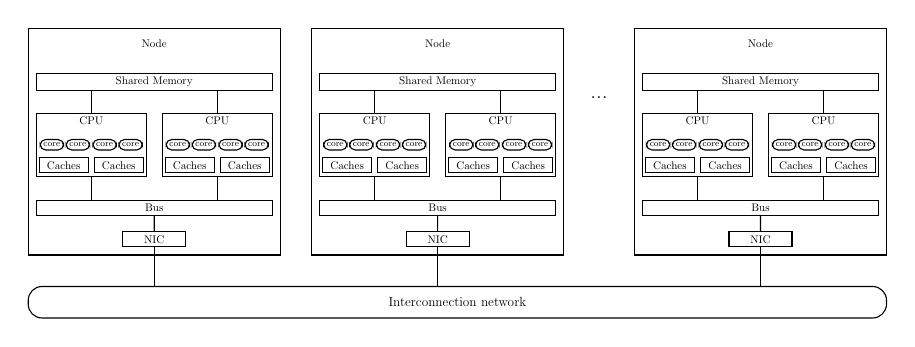
\begin{tikzpicture}[scale=0.4, every node/.style={scale=0.4}]

\pgfmathsetmacro{\lastxstart}{19}

\foreach \x[count = \i] in {-0.25, 8.75, \lastxstart} {
	\begin{scope}[xshift = \x cm]
	\draw (0.25,0) rectangle (8.25, 7.2);

	\node[draw, rectangle, minimum width = 2cm] (NIC\i) at (4.25, 0.5) {NIC};
	\node[draw, rectangle, minimum width = 7.5cm] (Bus) at (4.25, 1.5) {Bus};
	\node[draw, rectangle, minimum width = 7.5cm] (Shared) at (4.25, 5.5) {Shared Memory};
	\node at (4.25, 6.7) {Node};

	\begin{scope}[xshift = 2.25cm, yshift = -0.5cm]
	\node[rectangle, draw, minimum height = 2cm, minimum width = 3.5cm] (CPU1) at (0, 4) {};
	\node[below] at (CPU1.north) {CPU};

	\foreach \x in {-1.25, -0.425, 0.425, 1.25}
		\node[draw, rectangle, rounded corners = 2pt, inner sep = 3pt] at (\x, 4) {\footnotesize core};

	\foreach \x in {0.875, -0.875}
		\node[draw, rectangle, minimum width = 1.55cm] at (\x, 3.35) {Caches};
	\end{scope}

	\begin{scope}[xshift = 6.25cm, yshift = -0.5cm]
	\node[rectangle, draw, minimum height = 2cm, minimum width = 3.5cm] (CPU2) at (0, 4) {};
	\node[below] at (CPU2.north) {CPU};

	\foreach \x in {-1.25, -0.425, 0.425, 1.25}
		\node[draw, rectangle, rounded corners = 2pt, inner sep = 3pt] at (\x, 4) {\footnotesize core};

	\foreach \x in {0.875, -0.875}
		\node[draw, rectangle, minimum width = 1.55cm] at (\x, 3.35) {Caches};
	\end{scope}

	\draw (CPU1 |- Shared.south) -| (CPU1.north);
	\draw (CPU2 |- Shared.south) -| (CPU2.north);

	\draw (CPU1 |- Bus.north) -| (CPU1.south);
	\draw (CPU2 |- Bus.north) -| (CPU2.south);

	\draw (Bus) -- (NIC\i);
	\end{scope}
}

\pgfmathsetmacro{\lastx}{\lastxstart + 8.25}

\node[draw, rectangle, rounded corners = 5pt, minimum width = \lastx cm, minimum height = 1cm] (ICN) at ({\lastx / 2}, -1.5) {\large Interconnection network};

\draw (NIC1 |- ICN.north) -| (NIC1.south);
\draw (NIC2 |- ICN.north) -| (NIC2.south);
\draw (NIC3 |- ICN.north) -| (NIC3.south);

\node at (18.125, 5) {\huge ...};

\end{tikzpicture}
